\documentclass[11pt,a4paper]{article}

% Geometry
\usepackage{titling}
\setlength{\droptitle}{-7em}

% Timeline
\usepackage{chronosys}

% Code
\usepackage{minted}
\usemintedstyle{friendly}

% Tables
\usepackage{multicol}
\usepackage{multirow}
\usepackage{csquotes}
\usepackage{fullpage}

% Colors
\usepackage{xcolor, color, colortbl}
\colorlet{gray}{gray!70}
\colorlet{green}{green!50}
\definecolor{darkblue}{HTML}{1D577A}
\definecolor{rred}{HTML}{C03425}
\definecolor{darkgreen}{HTML}{8BB523}
\definecolor{ppurple}{HTML}{6B1B7F}
\definecolor{pblack}{HTML}{000000}
\definecolor{darkyellow}{HTML}{C0B225}

% Links
\usepackage{hyperref}
\definecolor{linkcolour}{rgb}{0,0.2,0.6}
\hypersetup{colorlinks,breaklinks,urlcolor=linkcolour,linkcolor=linkcolour,citecolor=blue}

% Graphics
\usepackage{graphics}
\graphicspath{{figures/}} % Location of the graphics files

% Title
\title{\textbf{Status Report \\ \small{Advanced Functional Programming}}}
\author{\small{Joris ten Tusscher, Cas van der Rest, Orestis Melkonian}}
\date{}

% Macros
\newcommand{\site}[1]{\footnote{\url{#1}}}
\newcommand{\icode}[1]{\mintinline{haskell}{#1}}
\newcommand\todo[1]{\textcolor{red}{#1}}

\begin{document}
\maketitle
%\vspace{-50pt}

\section{Techniques}

\subsection{Main Datatypes}
For representing music, we defined a highly-abstract \icode{Music} datatype, polymorphic to the specific elements of music manipulated through time. Hence, this datatype only specifies the operations invariant across all such specific representation, such as sequential/parallel composition of music and basic construction of music events or silence (of a certain duration), as shown below:

\begin{center}\begin{minipage}{0.5\textwidth}\begin{minted}[baselinestretch=1.1, fontsize=\small]{haskell}
data Music a = Music a :+: Music a
             | Music a :=: Music a
             | Note Duration a
             | Rest Duration
\end{minted}
\end{minipage}
\end{center}

For instance, in Western classical music it would appropriate to instantiate this type with an element representing
musical notes, represented as pairs of the pitch class (one of the 12 available ones) and the octave (how low/high is this note played). In South India's vocal tradition \textit{Konnakol}, on the other hand, one would only care about the rhythmic values (i.e. the durations), thus \icode{Music ()} would be more intuitive.

This freedom essentially enable us to choose the abstraction level we wish our music programs to be written in. Most importantly, we define a core representation \icode{MusicCore}, which is what every other abstraction should convert to, in order to allow for rendering/exporting in different formats. The typeclass is given below:

\begin{center}\begin{minipage}{0.5\textwidth}\begin{minted}[baselinestretch=1.1, fontsize=\small]{haskell}
class ToMusicCore a where
  toMusicCore :: Music a -> MusicCore
\end{minted}
\end{minipage}
\end{center}

We, naturally, focus on western music and define further helpful types/synonyms to represent common concepts encountered in music theory and practice (+ their conversions to \icode{MusicCore}). Furthermore, we provide operations often used in algorithmic music composition, such as transposition, inversion, mirroring, scaling and repetition. These are implemented as typeclasses, in order to allow user-defined \icode{Music} instances to extend them.

Last but not least, we provide commonly-used \textit{constants} of these musical concepts, such as popular scales/chords/durations.
\\ \\
For the generator DSL, we define a monadic interface that combines the \icode{State} and \icode{IO} monad: \icode{type MusicGenerator a = StateT GenState IO a}. In the future, this type might become polymorphic in the type of the state, but as of yet this is not the case. The \icode{GenState} type is defined as follows:
\begin{center}\begin{minipage}{0.7\textwidth}\begin{minted}[baselinestretch=1.1, fontsize=\small]{haskell}
data GenState = GenState { selector :: Selector
                         , pc       :: Entry PitchClass
                         , oct      :: Entry Octave
                         -- ... etc ...
                         }
\end{minted}
\end{minipage}
\end{center}

Where \icode{type Entry a = ([a], [Constraint a])}, representing all possible values for a certain type, and a list of constraints that are applied to that type. The type \icode{Selector} represents a function that selects a value from a list of possible values, and is defined as \icode{type Selector = forall a . [a] -> IO a}
\subsection{Libraries}
In order to avoid re-inventing the wheel, we utilized pre-existing Haskell libraries for exporting to MIDI/score formats. Specifically, we use \textbf{lilypond}\site{https://hackage.haskell.org/package/lilypond} to export music to Lilypond's digital score format, which can then be easily converted to PDF, etc... To enable MIDI export and music playback, we use \textbf{Euterpea}\site{https://hackage.haskell.org/package/Euterpea}. Since each of these libraries defines their own music datatype, integrating them entails converting from our \icode{MusicCore} type, which could be easily and naturally covered by the target types. For testing, we use HUnit\site{https://hackage.haskell.org/package/HUnit} and QuickCheck\site{https://hackage.haskell.org/package/QuickCheck}.

\section{Achievements}
Thus far, our main achievements are an extensive DSL for representing/transforming music and the ability to export in MIDI and score formats.
Design and implementation of the Generation DSL has started, but is still incomplete. Our code is available on Github\site{https://github.com/omelkonian/afp-project}.

\subsection{Music DSL}
We have implemented a rather expressive, but simple, EDSL for representing music and transformation. To give you a taste of the available operators, let us consider the example of expressing the harmonic progression of a famous song structure, known as the \textit{12-bar blues}. Given a particular tonic (i.e. note), one can derive 12 bars of chords, moving only between three basic (dominant) chords (I, IV and V) in a certain order. Moving from the tonic to the other ones is achieved simply by transposing a \icode{Chord} by a certain \icode{Interval}. The program expressing this structure is given below:
\begin{minted}[baselinestretch=1.1, fontsize=\small]{haskell}
-- Useful type synonyms
type Chord = [Pitch] ; type Melody = Music Pitch ; type Harmony = Music Chord
-- Abstract harmonic structure
bluesProgression :: Pitch -> Harmony
bluesProgression p =
  let tonic = p=|d7 <| wn
  in  line $ map ($ tonic) [id, id, id, id, (~> P4), (~> P4), id, id, (~> P5), (~> P5), id, id]
-- Concrete harmonic structure (Repeat C blues progression four times)
cBlues :: Harmony
cBlues = 4 ## bluesProgression (C#3)
\end{minted}
Given a way to improvise over such $D7$ chords, i.e. a function of type \icode{Chord -> Melody}, one could derive an improvisation line on top of this harmony, as demonstrated below:
\begin{minted}[baselinestretch=1.1, fontsize=\small]{haskell}
-- Parallel composition of harmonic progression and improvisation line (played an octave higher)
cBluesImprov :: Melody
cBluesImprov = chords cBlues :=: flatten (improviseOverD7 <$> cBlues) ~> P8
-- Create a line from a 4-note chord (we use postfix operators for silence)
improviseOverD7 :: Chord -> Melody
improviseOverD7 [a, b, c, d] =
  a <| qn :+: (b <~ Mi2) <| en :+: b <| en :+: (c <| qn :=: d <| qn) :+: (en~~) :+: d <| en
\end{minted}
We attached the generated score (i.e. \icode{writeToLilypond cBluesImprov}) in the Appendix.

\subsection{Generation DSL}
Goal of the generation DSL is to provide an interface for a programmer to quickly generate random pieces of music. We aim to enable the user to customize the generation process by either constraining which values can be generated, or by supplying functions that generate values for the appropriate types in place in place of just sampling them from their domain with uniform probability. We refer to the latter as \icode{Selector}, as they select values from a certain domain.
\subsection{Monadic Interface}
The generation DSL is provided as a monadic interface that a programmer can use to steer the generation process. The \icode{GenState} type contains the internal state of a generator, consisting of the types to generate for, and a \icode{Selector}, and can be manipulated through several library functions, on top of the functions that the generic \icode{StateT} interface provides.

A function \icode{runGenerator :: MusicGenerator a -> IO a} is provided that can be used to actually run a generator, alongside several functions that generate values for the data types used in our representation DSL. Below is a small example of a generator that generates a short melody.

\begin{minted}[baselinestretch=1.1, fontsize=\small]{haskell}
-- Generator execution
main :: IO ()
main =
  melody <- runGenerator randomMelody
  -- from here, you could export to a MIDO or score file

-- Generator definition
randomMelody :: MusicGenerator Melody
randomMelody = do
  notes <- replicateM 10 genNote    -- Generate random notes
  let melody = line notes           -- Combine into a melody
  return $ melody :+: invert melody -- Sequence melody with it's inversion
\end{minted}

As can be seen from the example above, the generator DSL integrates very nicely with the existing representation DSL. Furthermore, since the generator interface is a monad, generators can be manipulated in the same way as any other monad, making it very easy to compose larger, more complex generators from smaller ones.

\subsection{Future Extensions}
Although the basic structure for the generation DSL is in place, there is still quite a lot of work to do. Up until now, work on the generation DSL has mainly focused on finding a suitable approach. Now that we have one, we can start defining library functions that operate on the data types of the representation DSL. A few of the more notable parts of the DSL that we will be working on in the upcoming weeks are:
\begin{itemize}
\item
Suitable library functions for manipulating constraints, i.e. an intuitive way of adding (and removing) constraints from the generation process. We intend to add a \icode{local} function that will allow for partial generators to run under a different set of constraints without the need to remove and re-add all existing ones.
\item
The possibility to apply a custom \icode{Selector} to a generator to allow for non-uniform selection of values. The aim for this approach is to allow for many different possible ways of generating music besides complete randomness, such as chaos functions or L-systems. An added benefit is extensibility, as a programmer may come with their own procedure for determining appropriate musical values, which can then be applied to any \icode{MusicGenerator}.
\end{itemize}

Beside the extensions mentioned above, we also intend to include some small examples of applications for generators. Possibilities for this include automatically generating melodies over a certain chord progression or generating random exercises for certain scales or chords.

\section{Planning}
We are more or less on track with our initial planning, but we realised we cannot tackle Generation and Constraints separately. Thus, we decided to aim for a more integrated and iterative solution, where we gradually design/implement the GenDSL with constraints in mind. Since this task is not easily distributed amongst us, we will simultaneously work on GenDSL applications (i.e. chaotic systems, probabilistic rewriting grammars) from week 4 onwards, retrospectively adapting to new requirements we may encounter. Finally, the last week will be solely devoted to finalizing examples/applications.

\setupchronology{startyear=0, stopyear=6, startdate=false, stopdate=false, width=.9\hsize, height=.5cm, arrow=false}
\setupchronoperiode{textstyle=\bf\footnotesize}
\setupchronoevent{date=false, textstyle=\it\large, markdepth=1.5cm}
\chronoperiodecoloralternation{rred, darkgreen, rred, darkgreen}
\startchronology
\chronoevent{0}{Proposal(20/2)}
\chronoperiode{0}{2}{Music Representation}
\chronoperiode{2}{5}{Generation + Constraints + Applications}
\chronoevent{3}{Report(12/3)}
\chronoperiode{5}{6}{Applications}
\chronoevent{6}{Submission(5/4)}
\stopchronology

\newpage
\section*{\textsc{APPENDIX}: Generated Score for Blues Progression}
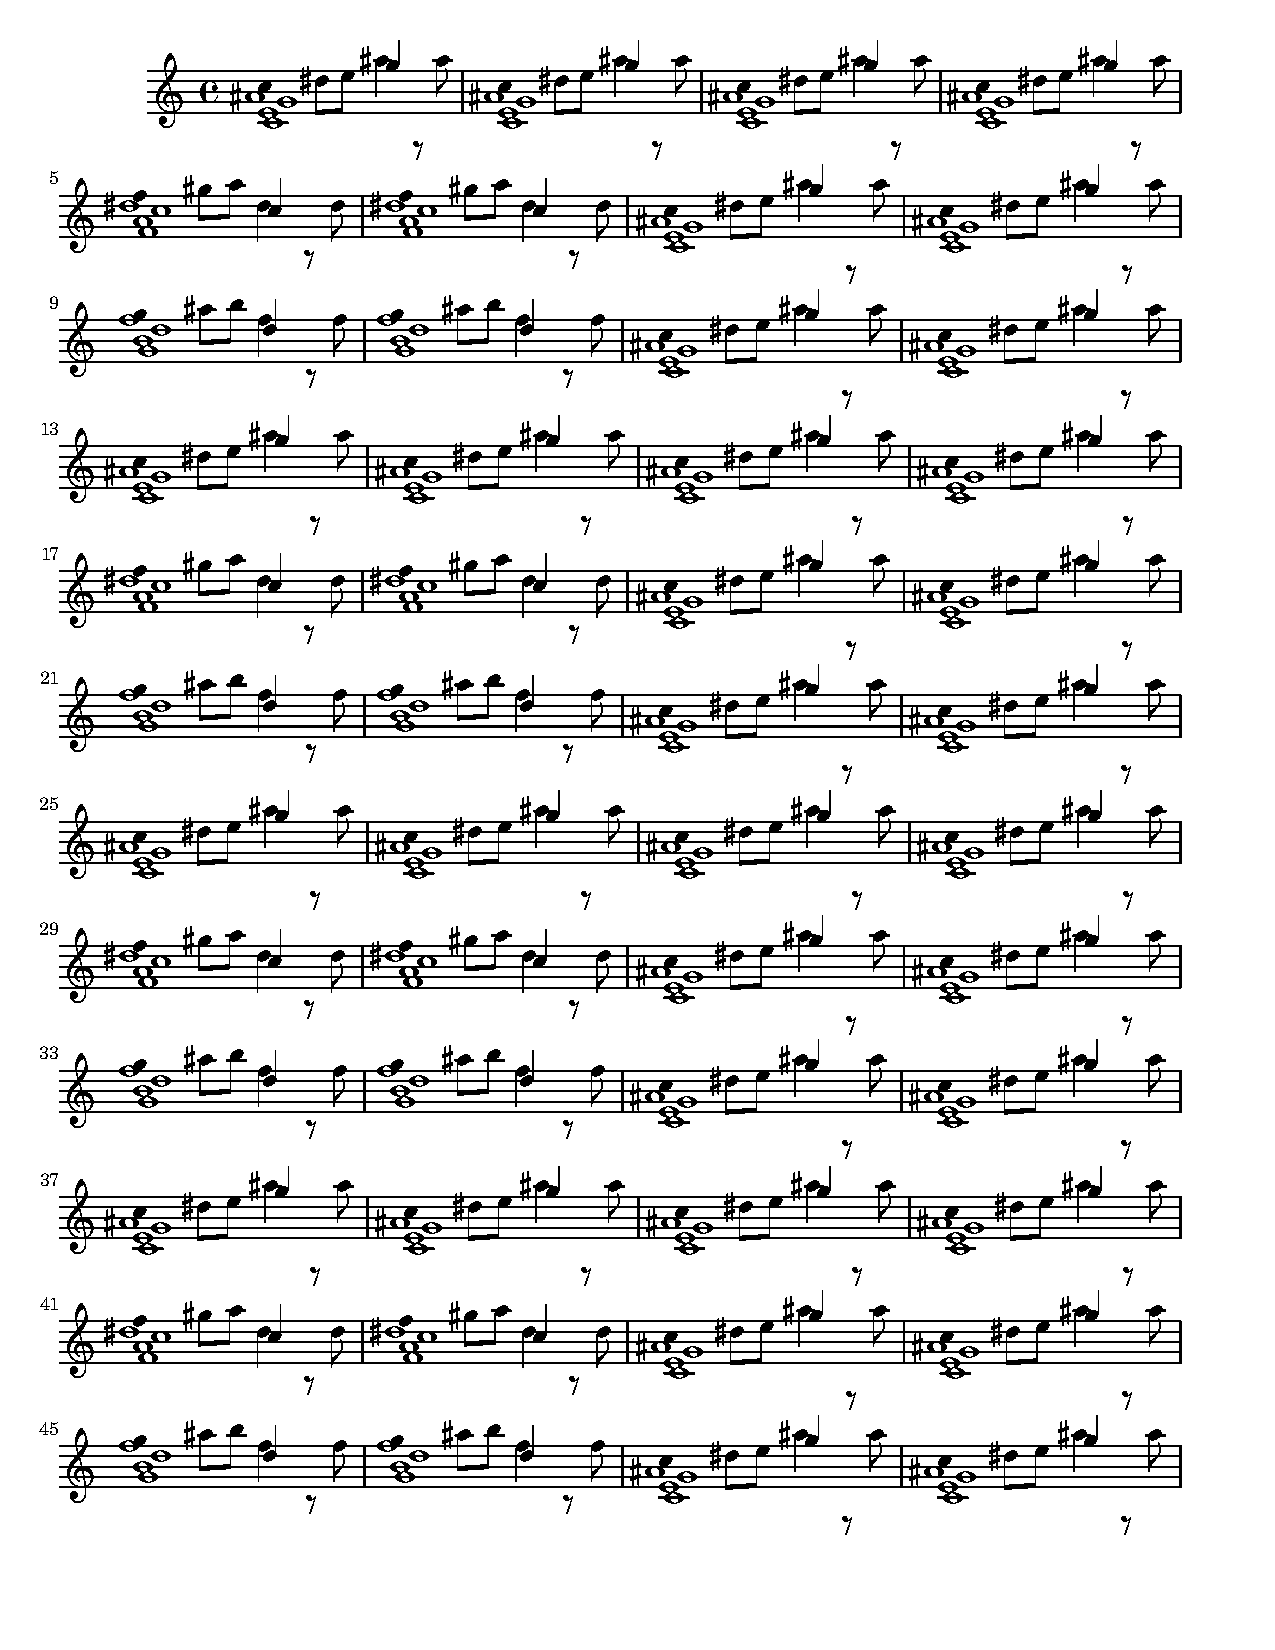
\includegraphics[scale=0.8]{blues.pdf}

\end{document}
